\documentclass[11pt,a4paper]{article}

\usepackage[utf8]{inputenc}
\usepackage[T1]{fontenc}
\usepackage{lmodern}
\usepackage{amsmath,amssymb}
\usepackage{graphicx}
\usepackage{booktabs}
\usepackage{siunitx}
\usepackage{hyperref}
\usepackage{xcolor}
\usepackage[margin=2.5cm]{geometry}
\usepackage{authblk}

\hypersetup{
  colorlinks=true,
  linkcolor=blue!50!black,
  citecolor=blue!50!black,
  urlcolor=blue!50!black
}

\title{Xenon TPCs for $\beta\beta0\nu$ searches}
\author{J.J.~G\'omez-Cadenas}
\date{\today}

\begin{document}
\maketitle

\begin{abstract}
We investigate the potential of xenon time-projection chambers (TPCs)
for neutrinoless double-beta decay ($\beta\beta0\nu$) searches.
\end{abstract}

\section*{Introduction}
\label{sec:intro}

Our initial goal is to reproduce the results obtained by the LZ
collaboration in their dedicated $\beta\beta0\nu$ sensitivity
study~\cite{LZ-bbonu}, using the detector description provided by the
LZ instrument paper~\cite{LZ-instrument} and the LZ Technical Design
Report~\cite{LZ-TDR}. Reproducing the LZ background model serves as
a validation of our Monte Carlo machinery before extrapolating to the
XLZD design.

\section{The LZ Detector}
\label{sec:lz}

\subsection{LZ Cryostat}
\label{sec:cryostat}

The LZ liquid-xenon payload is contained in a double-walled titanium
cryostat~\cite{LZ-instrument,LZ-TDR}. The Inner Cryostat Vessel (ICV)
holds the active LXe and the time-projection chamber; the Outer
Cryostat Vessel (OCV) provides the vacuum jacket and supports the ICV
through three tie-bar assemblies welded to its top head. Three legs
welded to the OCV bottom dished end carry the full assembly and also
host shelves for the lower acrylic vessels of the Outer Detector.

The entire cryostat is fabricated from a single 5-tonne slab of
ultra-radiopure ASTM Grade~1 titanium (TIMET batch HN3469, EBCH-melted,
0\% scrap), from which all plates, flanges, ports, and welding wires
were produced. Fabrication was carried out by Loterios (Milan) under
ASME BPVC~VIII~Div.~1.

The ICV has a 2:1 ellipsoidal top head, a cylindrical body that tapers
near half-height to reduce the passive LXe layer near the cathode, and
a 3:1 ellipsoidal dished bottom (chosen specifically to minimise the
LXe volume below the cathode). The vessel is split near the top by a
flange pair, and a stiffening ring at the top of the conical section
allows thinner walls (6--9~mm in the cylindrical region) while
remaining within ASME buckling limits. The OCV is segmented into three
flanged pieces (top head, middle cylinder, bottom head) so that each
fits in the Yates shaft. The full geometry is shown in
Fig.~\ref{fig:cryostat}.

\begin{figure}[h]
  \centering
  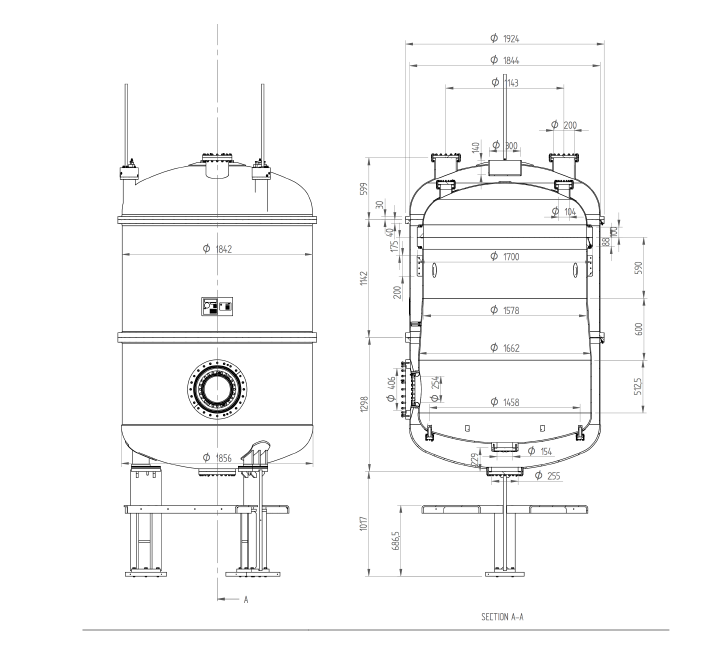
\includegraphics[width=0.85\textwidth]{cryostat.png}
  \caption{Engineering drawing of the LZ cryostat. Left: external view.
  Right: section A--A through the assembly, showing the ICV nested
  inside the OCV. Dimensions in mm.}
  \label{fig:cryostat}
\end{figure}

The bare titanium walls of the ICV and OCV weigh 950 and 1\,115~kg
respectively (TDR Table~5.4.1). The full cryostat assembly,
including all flanges, ports, tie bars, coldhead fins and welded
hardware, is taken to be \emph{2\,590~kg} for activity-budget
purposes, following Table~I of the LZ $\beta\beta0\nu$ sensitivity
paper~\cite{LZ-bbonu}; this is the value we adopt for normalisation
throughout this work. A summary of dimensions, masses, and the
late-chain $^{238}$U and $^{232}$Th specific activities used in the
background model is given in Table~\ref{tab:cryostat}.

\begin{table}[h]
  \centering
  \footnotesize
  \caption{LZ cryostat dimensions, masses and late-chain
  specific activities. Dimensions labelled ``drawing'' are read from
  the engineering drawing in Fig.~\ref{fig:cryostat}; ``TDR'' values
  come from~\cite{LZ-TDR}, Tables~1.2.1 and~5.4.1; masses and
  activities of the Ti vessel and insulation are taken from
  Table~I of~\cite{LZ-bbonu}. UL = upper limit. Values in italics
  are not separately tabulated in~\cite{LZ-bbonu} and are retained
  from the TDR Materials Table~9.2.7 for completeness.}
  \label{tab:cryostat}
  \begin{tabular}{ll}
    \toprule
    \multicolumn{2}{l}{\textbf{Inner Cryostat Vessel (ICV)}} \\
    \midrule
    Quantity                                    & Value \\
    \midrule
    Top neck flange ID                          & 1\,143~mm \\
    Upper region (top head) ID                  & 1\,700~mm \\
    Upper cylindrical body ID                   & 1\,662~mm \\
    Lower cylindrical body ID (after taper)     & 1\,578~mm \\
    Dished-end ID near cathode                  & 1\,458~mm \\
    Body ID (TDR cylindrical-section range)     & 1.58--1.66~m \\
    Height                                      & 2.59~m \\
    Wall thickness (top / upper / conical / lower / dished) & 7 / 9 / 9 / 9 / 11 mm \\
    Bare vessel mass                            & 950~kg \\
    \midrule
    \multicolumn{2}{l}{\textbf{Outer Cryostat Vessel (OCV)}} \\
    \midrule
    Body OD                                     & 1\,842--1\,844~mm \\
    Top flange OD                               & 1\,924~mm \\
    Bottom OD (at dished-end ring)              & 1\,856~mm \\
    Inside diameter                             & 1.83~m \\
    Total height                                & 3.04~m \\
    Wall thickness (top / side / dished)        & 8 / 7 / 14~mm \\
    Bare vessel mass                            & 1\,115~kg \\
    \bottomrule
  \end{tabular}

  \vspace{0.6em}

  \resizebox{\textwidth}{!}{%
  \begin{tabular}{lcccccc}
    \toprule
    \multicolumn{7}{l}{\textbf{Cryostat radioactivity (late-chain only)}} \\
    \midrule
    Component & Mass & $^{238}$U$_l$ & $^{232}$Th$_l$ & Total $^{238}$U$_l$ & Total $^{232}$Th$_l$ & Source \\
              & (kg) & (mBq/kg)      & (mBq/kg)       & (mBq)               & (mBq)                & \\
    \midrule
    Ti Cryostat Vessel    & 2\,590    & 0.08 (UL)              & 0.22 (UL)               & $\sim$207                  & $\sim$570                   & \cite{LZ-bbonu} Table~I \\
    Cryostat Insulation   & 13.8      & 11.1                   & 7.79                    & $\sim$153                  & $\sim$107                   & \cite{LZ-bbonu} Table~I \\
    \emph{Cryostat Seals} & \emph{33.7} & \emph{26.2}          & \emph{4.24}             & \emph{$\sim$883}           & \emph{$\sim$143}            & \emph{TDR Table~9.2.7} \\
    \emph{Cryostat Teflon Liner} & \emph{26} & \emph{0.02}     & \emph{0.03}             & \emph{$\sim$0.5}           & \emph{$\sim$0.8}            & \emph{TDR Table~9.2.7} \\
    \bottomrule
  \end{tabular}%
  }
\end{table}

\appendix

\section{Cryostat geometry and mass budget for the simulation}
\label{app:cryostat-model}

This appendix describes the cryostat representation used in the
present simulation. It supersedes the simple-cylinder plus
averaged-endcap model that was inherited from earlier LZ analyses,
in which the OCV and ICV ellipsoidal heads were lumped into two
mass-weighted endcap sources and the missing $\sim 1160$~kg of
hardware mass was absorbed into a single ``extra Ti'' surface
source on the bottom endcap.

\subsection{Motivation}

Reference~\cite{LZ-bbonu} (Table~I) gives the full Ti cryostat
assembly mass as $2\,590$~kg with late-chain specific activities
of 0.08~mBq/kg ($^{238}$U-late) and 0.22~mBq/kg
($^{232}$Th-late). To reproduce that paper's background budget
the model used here must carry the same total Ti activity, that
is, the same total Ti mass at the same specific activity. The
TDR's bare-vessel masses (Table~5.4.1 of~\cite{LZ-TDR}) are
$950$~kg (ICV) and $1\,115$~kg (OCV); a simple-cylinder
geometric model with the wall thicknesses of
\texttt{data/lz\_cryo\_geometry.csv} gives $1\,433$~kg for the two
vessels combined. The remaining $\sim 1\,160$~kg is real Ti
hardware --- flanges, ports, support legs, stiffeners, coldhead
fins, and internal anchor rings --- that the simple-cylinder
model omits. The new model places every gram of Ti at a defined
geometric location, so each kilogram has a birth point for MC
photon emission; nothing is treated as phantom mass.

\subsection{Geometry primitives}

Two pure-geometry types are introduced. \texttt{GCyl} is a
cylindrical shell with axis along $\hat{z}$, characterized by
inner radius $R_i$, radial wall thickness $t$, and axial extent
$[z_{\min}, z_{\max}]$. \texttt{GDisk} is a head/disc attached to
a cylinder of equatorial radius $R$ at axial position $z_{\rm
eq}$, with shape parameter $n$ (the head depth equals $R/n$;
$n = \infty$ is a flat disc, $n = 1$ a hemisphere, $n = 2$ a 2:1
ellipsoidal head, $n = 3$ a 3:1 head) and an outward direction
($\uparrow$ or $\downarrow$). Both types expose a uniform
interface --- area, volume, mass given a material density,
uniform-on-surface point sampling, inward normal, and ray
path-length through the shell --- used both by the analytic
shielding integrals and by the per-photon Monte Carlo.

\subsection{Cryostat composition}

The composite \texttt{Cryostat} object is built from two CSV
files. The geometry file
\texttt{data/lz\_cryo\_geometry.csv} contains two rows (OCV and
ICV) with the radius, total height, cylindrical-section height,
wall and head thicknesses, and head aspect ratios; each row
generates one \texttt{GCyl} (the cylindrical body) and two
\texttt{GDisk} (top and bottom heads). The extras file
\texttt{data/lz\_cryo\_extras.csv} contains 22 rows representing
all the additional Ti hardware identified from the
LZ-TDR~\cite{LZ-TDR} and from the engineering drawing
(\texttt{docs/cryostat.png}). Each extras row encodes an annular
\texttt{GCyl} together with a category label, a multiplicity
\texttt{count} (for items that appear $N$ times at different
azimuths, such as the three OCV legs or the six coldhead fins),
and a flag \texttt{include\_in\_mc} that selects whether the row
is used as a $\gamma$-source ring in the Monte Carlo.

The 22 extras break down by category as: 5 flanges, 8 port
entries (12 individual pieces), 1 support-leg entry (3 pieces),
1 stiffener, 1 coldhead-fin entry (6 pieces), and 5
internal-anchor-ring entries.

\subsection{Mass budget}

Computed with $\rho_{\rm Ti} = 4.510$~g/cm$^3$:

\begin{table}[h]
  \centering
  \footnotesize
  \caption{Ti mass budget of the cryostat model. Categories beyond
  the barrels and heads are read from
  \texttt{data/lz\_cryo\_extras.csv}.}
  \label{tab:cryostat-budget}
  \begin{tabular}{lr}
    \toprule
    Category & Mass (kg) \\
    \midrule
    Barrels (OCV + ICV)             & 791  \\
    Heads (4 ellipsoidal)           & 642  \\
    Flanges (5 entries)             & 606  \\
    Ports (8 entries, 12 pieces)    & 121  \\
    Legs (3 pieces)                 & 122  \\
    Stiffener                       &  26  \\
    Coldhead fins (6 pieces)        &  57  \\
    Internal anchor rings (10 pieces) & 208  \\
    \midrule
    \textbf{Total Ti mass (model)}  & \textbf{2\,572}  \\
    bb0nu Table~I~\cite{LZ-bbonu}   & 2\,590  \\
    Residual (model $-$ bb0nu)      & $-18$~kg ($-0.7\%$) \\
    \bottomrule
  \end{tabular}
\end{table}

The agreement with~\cite{LZ-bbonu} is at the $1\%$ level. The
test \texttt{test/test\_geometry2.jl} regresses against $\pm 5\%$
tolerance.

\subsection{Radioactive (MC-active) subset}

Not all of the 22 extras are exposed as MC sources. Items whose
geometry does not fit the axisymmetric \texttt{GCyl} primitive
cleanly (the three OCV legs are off-axis), or which are buried
inside other Ti walls (internal anchors, the ICV stiffening
ring, the six coldhead fins), or which are small enough that
their contribution to the fiducial volume is sub-percent (the
weir drains, the ICV bottom anchor port flanges, the OCV bottom
small port) are flagged \texttt{include\_in\_mc = false}. The
radioactive model comprises the barrels, the four heads, the
five flanges, and the six main ports (HV port, cathode-side
port, YBe recess, conduit ports, tie-bar ports, and bottom
umbilical), totalling $2\,144$~kg --- $83\%$ of the full Ti
budget. The remaining $17\%$ ($428$~kg) consists almost entirely
of items that are heavily shielded or geometrically hidden, so
its contribution to the FV background is expected to be
considerably less than $17\%$.

\begin{figure}[h]
  \centering
  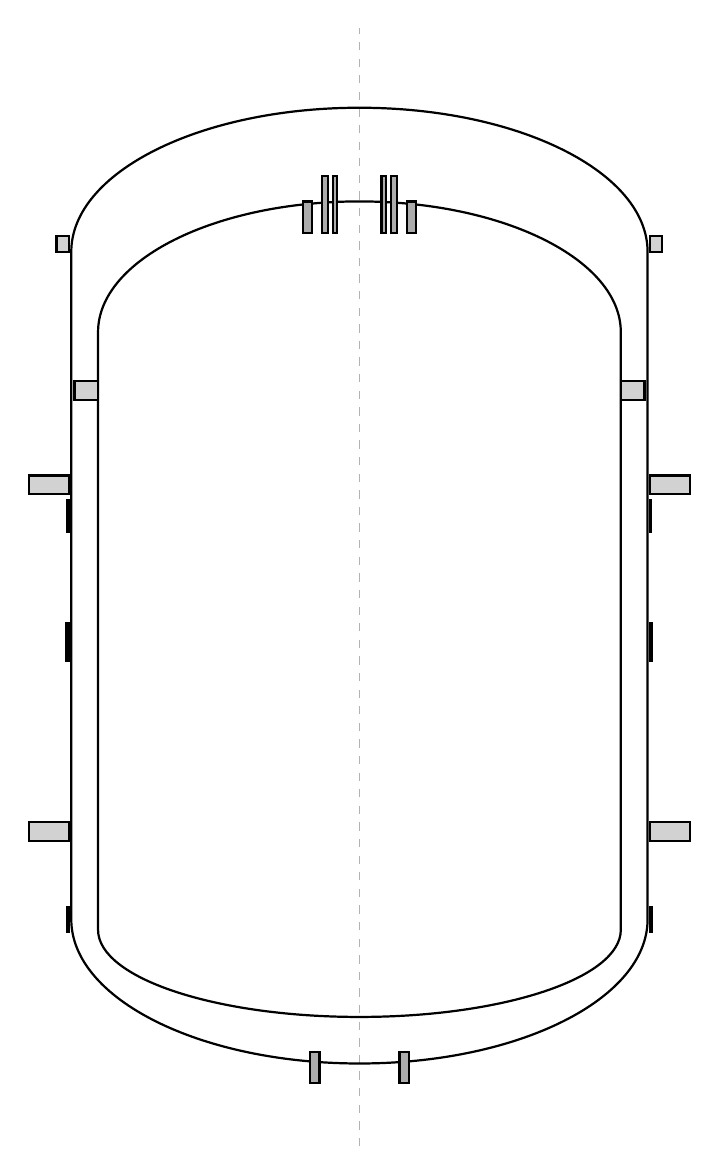
\includegraphics[width=0.55\textwidth]{lz_cryo_model.png}
  \caption{Section view of the LZ cryostat radioactive model: the
  two outer contours (OCV with 2:1 top and 2:1 bottom; ICV with
  2:1 top and 3:1 bottom), the five flanges (light fill), and the
  six main ports (darker fill). MC-inactive structural elements
  (legs, stiffener, coldhead fins, internal anchor rings, weir
  drains, ICV anchor port flanges, OCV bottom small port) are
  intentionally omitted.}
  \label{fig:cryo-model}
\end{figure}

\subsection{Conventions and caveats}

Lengths in cm, masses in kg, $z = 0$ at the cathode (TPC drift
region $z \in [0, 145.6]$~cm). Cylindrical-shell volumes use the
exact formula $\pi(R_o^2 - R_i^2)\,H$; head volumes use the
thin-shell approximation $A_{\rm inner} \times t$, with relative
error $\mathcal{O}(t/R) \approx 1\%$ at LZ scales. Flange axial
thicknesses and most port axial extents are estimates from
ASME-typical values for Ti at 1.8~m diameter / 2~bar internal
pressure: the engineering drawing gives reliable diameters but
not flange thicknesses. The two side ports (HV, cathode-side)
have axes perpendicular to $\hat{z}$ and are encoded as thin
annular rings at the OCV body radius --- a representation that
conserves mass and places the source at the correct $(R, z)$ but
does not capture the radial port axis. Items appearing $N$ times
at different azimuths share one CSV row with \texttt{count $= N$};
the loader produces $N$ copies at the same $(R, z)$, which is
exact for axisymmetric mass and shielding integrals.

\begin{thebibliography}{9}

\bibitem{LZ-bbonu}
LZ Collaboration,
\emph{Projected sensitivity of the LUX-ZEPLIN experiment to the
$0\nu\beta\beta$ decay of $^{136}$Xe},
Phys.~Rev.~C \textbf{102}, 014602 (2020),
arXiv:1912.04248.

\bibitem{LZ-instrument}
LZ Collaboration,
\emph{The LUX-ZEPLIN (LZ) experiment},
Nucl.~Instrum.~Meth.~A \textbf{953}, 163047 (2020),
arXiv:1910.09124.

\bibitem{LZ-TDR}
LZ Collaboration,
\emph{LUX-ZEPLIN (LZ) Technical Design Report},
arXiv:1703.09144 (2017).

\end{thebibliography}

\end{document}
